\documentclass[12pt]{article}
\usepackage{epsfig}
\usepackage{graphicx}
\usepackage{color}
\usepackage[frenchb]{babel}
\usepackage{subfigure}
\usepackage{algorithm}
\usepackage{algpseudocode}
\usepackage{amsmath}
\usepackage{url}
\usepackage{listings}


% Pour pouvoir utiliser les accents directement dans LaTeX, sans utiliser les commandes \'
%\usepackage[latin1]{inputenc} % entree 8 bits iso-latin1
\usepackage[utf8]{inputenc} % entree 8 bits utf8, fonctionne avec MikTeX sur Windows.
\usepackage[T1]{fontenc}      % encodage 8 bits des fontes utilisees

% Pour agrandir les marges
\addtolength{\oddsidemargin}{-.875in}
\addtolength{\evensidemargin}{-.875in}
\addtolength{\textwidth}{1.75in}
\addtolength{\topmargin}{-.875in}
\addtolength{\textheight}{1.75in}

\makeatletter\renewcommand{\ALG@name}{Algorithme}


\begin{document}
\title{GLO-4001 Introduction à la robotique mobile \\  TP1 \\ 23 octobre 2017}
\author{Alexandra Mercier et Alexandre Gingras-Courchesne}
\maketitle


{\bf Attention! N'oubliez pas d'attacher le code de toutes les questions dans la remise .zip de votre travail. Si les codes sont manquants, nous pourrons retirer jusqu'à 20\% de la note. }

Pour tous les étudiants, vous devez fournir un rapport en un seul document (format pdf) et les fichiers matlab ou Python zippé. Pour toutes les questions, n'oubliez pas de mettre le détail des calculs.

% ================== Carte =======================
\section{Carte 2D à partir d'un gyroscope et d'un capteur de distance (15 pts)}

\subsection{Carte 2D locale (5 pts)}
\label{CarteLocale}

\subsubsection{Calculs}
Pour pouvoir créer un nuage de point sur un plan 2D, il faut utiliser nos données pour obtenir une variété de points x, y.
Pour cela, il faut:
\begin{enumerate}
        \item Convertir la tension de notre capteur en distance.
        \item Convertir la vitesse angulaire du gyroscope en angle.
        \item Obtenir un point (x, y) avec la distance et l'angle.
\end{enumerate}

\textbf{Convertir la tension du capteur}
Soit la fonction du capteur avant bruit:
\[ z(d) = 1/d \]

Comme le capteur est bruité, il faut consid\'erer celui-ci. On mod\'elise donc la fonction avec une gaussienne:

\textbf{Convertir la vitesse angulaire}
Soit :
\[ \frac{d\theta}{dt} = g \] o\`u g est la vitesse angulaire.
On peut approximer cela \`a:
\[ \frac{\Delta \theta}{\Delta t}  = g\]
Avec le temps t noté, on peut trouver la valeur de $\theta$ en ajoutant $\Delta t * g $ ou $ (t_{valeur précédente} - t_{valeur courante}) * g$.

Toutefois, cette technique va cumuler de l'erreur avec le temps.
Pour Réduire l'erreur du à l'intégration:

\textbf{Obtenir un point (x, y)}

Soit avec la trigonométrie:
\[ x = d*\cos(\theta) \] \[ y = d*\sin(\theta) \]

\subsubsection{Code}
Le fichier question1.py contient le code utilisé pour former la carte 2D.
\subsubsection{Carte}

\begin{figure}[ht]
 \begin{center}
  \begin{tabular}{c}
    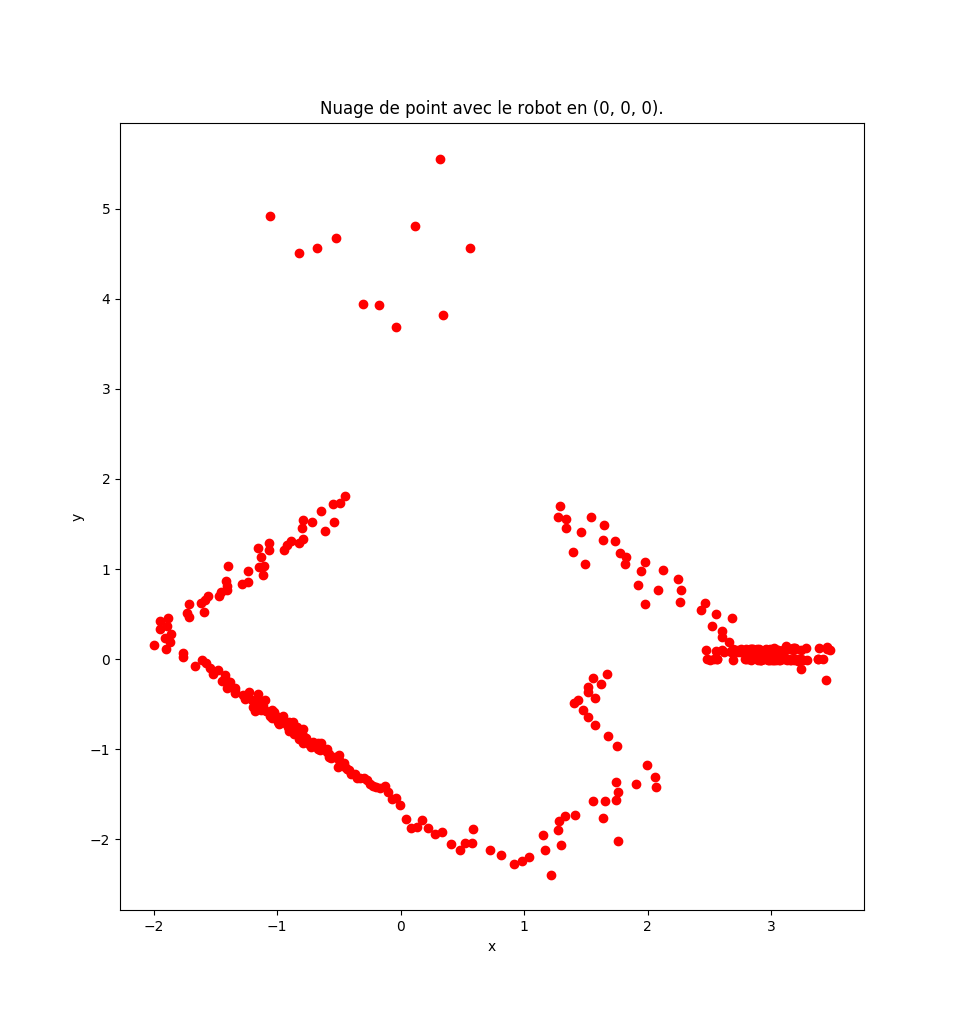
\includegraphics[width=0.75\textwidth]{q1-carte-local.png}
  \end{tabular}
 \end{center}
\vspace{-0.25in}
 \caption{Carte 2D générée avec les données matlab et le code python.}
    \label{carte-2d-locale}
\end{figure}

La figure \ref{carte-2d-locale} représente le nuage de point.

\newpage
\subsection{Localisation du robot dans la carte globale (10 pts)}

\subsubsection{Calculs}
\textbf{Création de $P_{Homogene}$:}

\[ \text{Soit } P_{Homogene} =
\begin{bmatrix}
    x_1 & x_2 & x_3 & ... & x_n \\
    y_1 & y_2 & y_3 & ... & y_n \\
    1   & 1   & 1   & ... & 1   \\
\end{bmatrix}
\]

\textbf{D\'etermination des matrices de transformation T:}

Soit pour faire une translation $[T_x, T_y]$, il faut multiplier $P_{Homogene}$ par la matrice

\[
    T =
    \begin{bmatrix}
        1 & 0 & T_{x} \\
        0 & 1 & T_{y} \\
        0 & 0 & 1
    \end{bmatrix}
    \]

\textbf{D\'etermination des matrices de transformation R:}

Soit pour faire une rotation de $\theta rad$, cela \'equivaut \`a multiplier par la matrice
\[
    R =
    \begin{bmatrix}
        \cos{\theta} & -\sin{\theta} & 0 \\
        \sin{\theta} & \cos{\theta} & 0 \\
        0 & 0 & 1 \\
    \end{bmatrix}
    \]

\subsubsection{Code}


\subsubsection{Réponse}

% ================== CAMERA =======================
\newpage
\section{Modèle de caméra et positionnement par caméra}

\subsection{Génération d'une image (5 pts)}
\label{generation_image}
\subsubsection{Calculs}
Soit la relation entre le point correspondant [u, v] et la position dans le monde r\'eel $ [L_{ix}, L_{iy}, L_{iz}] $
\[ \left[ {\begin{array}{c}
                u \\
    v \\ \end{array} } \right] =
    \frac{f}{L_{iz}}
    \left[ {\begin{array}{c} L_{ix} \\ L_{iy} \\ \end{array}} \right]
\]

Comme la valeur $L_y$ est nulle, nous obtenons:


\[ \left[ {\begin{array}{c}
                u \\
    v \\ \end{array} } \right] =
    \frac{f}{L_{iz}}
    \left[ {\begin{array}{c} L_{ix} \\ 0 \\ \end{array}} \right]
=
    \left[ {\begin{array}{c} \frac{f}{L_{iz}} * L_{ix} \\ \frac{f}{L_{iz}} * 0 \\ \end{array}} \right]
=
    \left[ {\begin{array}{c} \frac{f}{L_{iz}} * L_{ix} \\ 0 \\ \end{array}} \right]

\]

On peut ainsi en conclure que:
\[
    u =  \frac{f}{L_{iz}} * L_{ix}
\]
\[
    v = 0
\]
o\`u u et v sont en pixels, et f = 1200 pixels.

\subsubsection{Code}

Le fichier question2.py contient la fonction make_image_uv_pose qui convertie la position de $L_i$ en une position d'écran [u, v].

\subsection{Estimation de la pose de la caméra à partir des angles $\alpha$ et $\beta$ (5 pts)}
\subsubsection{Calculs}
\subsubsection{Code}
\subsubsection{Réponse}

\subsection{Impact du bruit sur l'estimation des repères (10 pts)}
\subsubsection{Calculs}
\subsubsection{Code}
\subsubsection{Réponse}

% ================== STEREO =======================
\newpage
\section{Imagerie stéréo  (15 pts)}

\subsection{Distance focale $f$ (4 pts)}
\subsubsection{Calculs}
Pour obtenir f, il faut connaître les valeurs [u, v] de la tour verte.
Mesur\'ee avec une r\`egle, on obtient:
\[ u = 0 px \text{(centre de l'image)}\]
\[ v = 310 px\]
Sachant que:
\[ \text{Axe des v: } 0.7cm = 200px \]
En reprenant la fonction trouv\'ee en \ref{generation_image}, on sait que :

\[
    u =  \frac{f}{L_{iz}} * L_{ix}
\]
\[
    v =  \frac{f}{L_{iz}} * L_{iy}
\]
On isole $f$ dans l'\'equation de v:
\[
    f =  \frac{v * L_{iz}}{L_{iy}}
\]

Comme on sait que la tour fait 15cm de hauteur ($L_{iy} = 15$) et que celle-ci est \`a une distance de 95cm de la cam\'era ($L_{iz} = 95$):
\[
    f =  \frac{v * L_{iz}}{L_{iy}} = \frac{310px * 95 cm}{15cm} = 1963.33 px = 2000 px
\]


\subsubsection{Code}
\subsubsection{Réponse}
La distance focale est d'environ 2000 pixels.

\subsection{Estimation de la distance $A_z$ de chaque tour LEGO (6 pts)}
\label{estimation_distance_Az}
\subsubsection{Calculs}

\begin{table}[h]
\caption{Disparit\'e $d$ mesur\'ee avec la r\`egle}
\label{TableCoord}
\begin{center}
\begin{tabular}{|c|c|c|c|}
\hline
    tour   &  $u_{gauche}$  &  $u_{droite}$  &  $d$ $(u_g - u_d)$ \\
\hline
    rouge  & --1.75cm & -2.65cm & 0.90cm \\
    bleu   & 1.70cm & 0.50cm & 1.20cm \\
    jaune  & 2.50cm & 1.65cm & 0.85cm \\
\hline
\end{tabular}
\end{center}
\end{table}

Pour convertir la disparit\'e en pixels, on utilise la r\`egle de de trois sachant que:

\[ \text{Axe des u:} 1.2cm = 200px \]


\begin{table}[h]
\caption{Disparit\'e $d$ en pixels}
\label{TableCoord}
\begin{center}
\begin{tabular}{|c|c|c|c|}
\hline
    tour   &  $d$ \\
\hline
    rouge  &  150px \\
    bleu   &  200px \\
    jaune  &  140px \\
\hline
\end{tabular}
\end{center}
\end{table}

On peut trouver $A_z$ avec la formule:
\[ A_z = \frac{f \dot b}{d}\]
Avec f = 2000px et b = 5cm.

\subsubsection{Code}
\subsubsection{Réponse}

\begin{table}[h]
\caption{Distance en $z$ des centres des faces des colonnes.}
\label{TableCoord}
\begin{center}
\begin{tabular}{|c|c|}
\hline
 tour   & $A_z$ \\
\hline
 rouge  & 67cm \\
 bleu   & 50cm \\
jaune   & 71cm \\
\hline
\end{tabular}
\end{center}
\end{table}


\subsection{Estimation de la coordonnée $A_x$ de chaque tour LEGO (5 pts)}
\subsubsection{Calculs}
On r\'eutilise les valeurs de $u_{gauche}$ mesur\'ees en \ref{estimation_distance_Az}.
Puis, on les convertie en pixels.

\begin{table}[h]
    \caption{$u_{gauche}$ en pixels}
\label{TableCoord}
\begin{center}
\begin{tabular}{|c|c|}
\hline
    tour   &  $u_{gauche}$\\
\hline
    rouge  & -290px  \\
    bleu   & 280px   \\
    jaune  & 420px   \\
\hline
\end{tabular}
\end{center}
\end{table}

Avec la trigonométrie, on peut conlure que $u_{gauche} \propto A_x$ soit :
\[ u_g = \frac{f}{A_z}A_x\]
\[ A_x = \frac{u_g \dot A_z}{f} \]
Sachant que $f = 2000px$ et en utilisant les valeurs de $A_z$ trouvées en \ref{estimation_distance_Az}.

\subsubsection{Code}
\subsubsection{Réponse}

\begin{table}[h]
\caption{Coordonnée en $x$ des centres des faces des colonnes.}
\label{TableX}
\begin{center}
\begin{tabular}{|c|c|}
\hline
 tour   &  $A_x$ \\
\hline
 rouge  &  -9.7cm     \\
 vert   &  0.0cm  \\
 bleu   &  7.0cm    \\
 jaune  &  15cm     \\
\hline
\end{tabular}
\end{center}
\end{table}


% ==================  FAST =======================
\newpage
\section{Extracteur de coin FAST (13 pts)}
 \label{SectionFAST}

\subsection{Fonction d'extraction des coins FAST (7 pts)}
\subsection{Test de votre fonction \texttt{DetectionCoinFAST} sur une image réelle (6 pts)}
% ================== Descripteur BRIEF =======================

\newpage
\section{Descripteur BRIEF (17 pts pour GLO-4001, 27 pts pour GLO-7021)}

\subsection{Fonction calculant un descripteur BRIEF (3 pts)}

\subsection{Appariement features image gauche-droite (5 pts)}
 Appliquez votre pipeline sur les images suivantes :
 \begin{itemize}
 \item \texttt{bw-rectified-left-022146small.png} et
 \item \texttt{bw-rectified-right-022146small.png},
 \end{itemize}
\end{document}
